\subsection{Fravælgelse gestik-par}
\label{TestresultaterSkiftDaarlig}
%
I følgende afsnit analyseres hvilke af de syv semaforiske gestik-par testpersonerne fravælger samt hvorfor testpersonerne netop fravælger disse gestik-par. På baggrund af analysen bør det være muligt at udpege hvilke semaforiske gestikker, der hvertfald ikke skal knyttes til at skifte musiknummer. Analysen bygger på testpersonerne respons til spørgsmålet: \textit{Hvilken gestik kan du mindst lide? og hvorfor?}, hvor testpersonernes samlede data er vedlagt i ELEKTRONISK BILAG.
%
\begin{figure}[H]
	\centering
	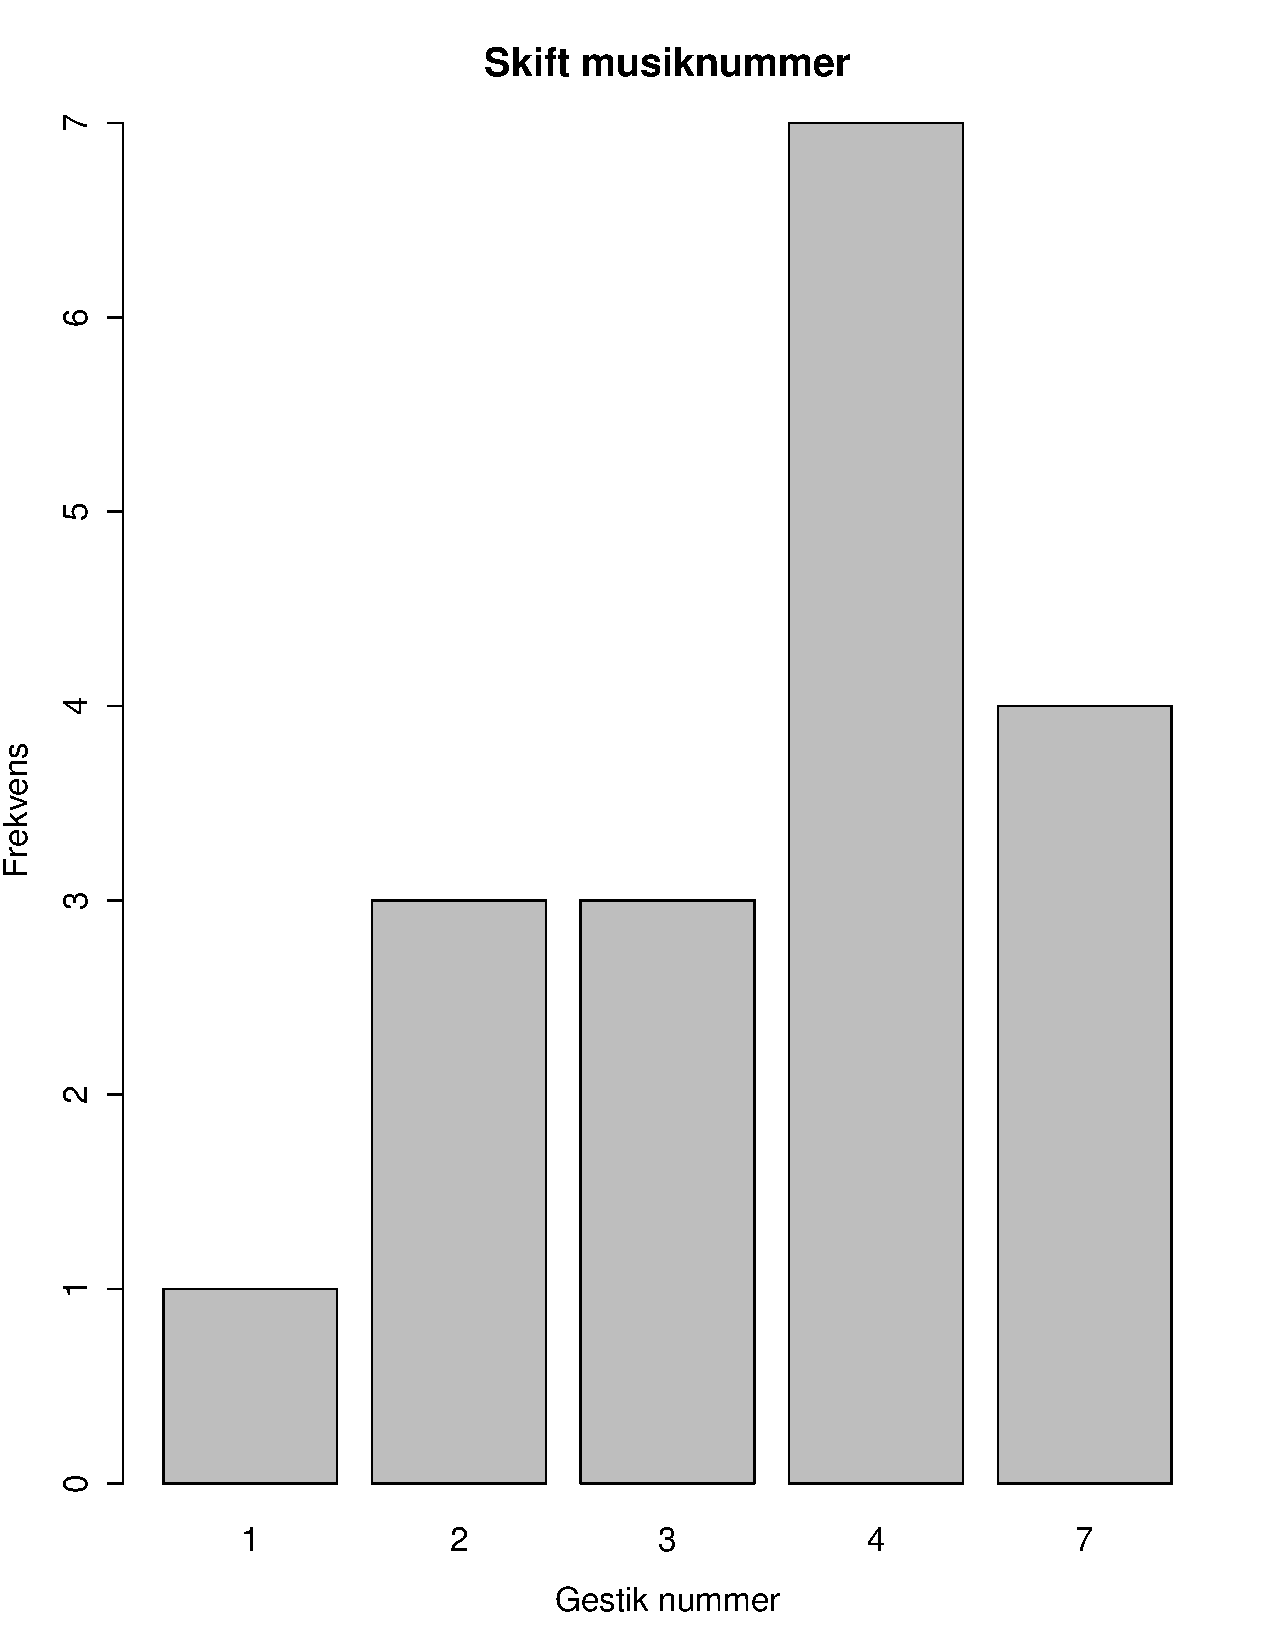
\includegraphics[resolution=300,width=0.5\textwidth]{Test1/DatabehandlingGrafer/DaarligstGestikSkift.pdf}
	\caption{Barplot over hvilke gestik-par testpersonerne fravælger i forbindelse med at skifte musiknummer frem og tilbage. Søjlerne bygger på testpersonernes respons, hvorfor det kun er de fravalgte gestik-par, der udgør plottet.}
	\label{fig:DaarligstGestikSkift}
\end{figure}
\noindent
%
På \autoref{fig:DaarligstGestikSkift} fremgår det hvilke gestik-par de 18 testpersoner fravælger i forbindelse med at skifte musiknummer. Det fremgår tydeligt at gestik-par 4 er det par, som flest testpersoner fravælger i forhold til de resterende par på \autoref{fig:DaarligstGestikSkift}. Årsagen til at testperson 14 har valgt gestik-par 1, som værende den testpersonen mindst kan lide, begrundes med at testpersonen forestiller sig, at det er en bevægelse testpersonen vil komme til at gøre gentagende gange foran sit anlæg eller under en samtale. Testperson 1, testperson 5 og testperson 16 har alle valgt gestik-par 2, som værende den de mindst kan lide, fordi gestikken er modsat af, hvad de forventer er frem og tilbage. At gestik-par 3 fravælges begrunder testperson 3, testperson 11 og testperson 13 med at hvis der skulle peges i en retning så skulle det være med pegefingeren og ikke tommelfingeren, det er en akavet bevægelse og fordi gestikken er statisk. I den forbindelse kommenterer testperson 5 at vedkommende heller ikke bryder sig om hverken gestik-par 3 eller gestik-par 7, netop fordi de er statiske.

Der er forskellige årsager til at syv testpersoner fravælger gestik-par 4. Testperson 4 og testperson 6 fravælger gestikken fordi den er mærkelig, hvor testperson 4 forbinder det med at skulle tage telefonen. Testperson 8 forstår ikke hvorfor det er lige præcis er det håndtegn der skal bruges. Testperson 10 oplever ikke at gestikken bringer noget nyt men snarre er en besværlig version af gestik-par 5. I forhold til håndtegnet i gestik-par 4, så kommenterer testperson 12 at det er unaturligt at gøre noget med lillefingere, testperson 7 kommenterer dels at det er en stor armbevægelse og dels at det er et sjovt håndtegn, som vil blive glemt, hvis det ikke bliver brugt. I tillæg kommenterer testperson 18 ligeledes at det er en unaturlig gestik, som vil blive glemt dog pointerer testpersonen at det er en effektiv gestik i og med at den ikke vil blive lavet ved en fejl. 

Årsagen til at gestik-par 7 fravælges skyldes ifølge testperson 2, testperson 9 og testperson 17, dels at den virkede mærkelig, dels at den ikke blev opfattet og dels at den minder lidt om en pistol. Ligesom gestik-par 3 blandt andet blev fravalgt fordi den er statisk, så fravælger testperson 15 af samme årsag gestik-par 7 og fordi det er et enkelt tegn.\blankline
%
For at afgøre hvilke af de syv gestik-par, der skal fravælges er det nødvendigt at sammenholde hvilke gestikker testpersonerne fravælger med de gestikker, som indgår i testpersonernes top tre rangering. Der opstilles derfor en tabel over de fire fravalgte gestik-par og hvordan de indgår i testpersonernes rangering.    
%
\begin{table}[H]
	\centering
	\begin{tabular}{ | p{1.5cm} | p{2.1cm} | p{2.1cm} | p{2.1cm} | p{2.1cm} | p{2.1cm} |}
	\hline
		 & Gestik-par 1 & Gestik-par 2 & Gestik-par 3 & Gestik-par 4 & Gestik-par 7 \\ \hline
		1. Plads & 10 & 3 & 1 & 0 & 0\\ \hline
		2. Plads & 2 & 3 & 3 & 0 & 1\\ \hline
		3. Plads & 0 & 0 & 7 & 5 & 2\\ \hline
	\end{tabular}
	\caption{Oversigt over hvor ofte og hvor de fem fravalgte gestikker indgår i testpersonernes top tre rangering.}
	\label{tab:FravalgteTopTreSkift}
\end{table}
\noindent
%
På baggrund af \autoref{tab:FravalgteTopTreSkift} sammenholdt med \autoref{fig:DaarligstGestikSkift}, tyder det på at gestik-par 4 og gestik-par 7 kan ekskluderes fra fremtidige undersøgelser. Det skyldes at selvom gestik-par 4 indgår fem gange i testpersonernes top tre, så fravælges parret af syv testpersoner. Derudover tyder det på, at de fem testpersoner, som har inkluderet gestik-par 4 i deres top tre, har gjort det på baggrund af bevægelsen snarre end kombinationen af både håndtegnet og bevægelsen. Gestik-par 7 ekskluderes da parret kun indgår tre gange i top tre og da den derudover fravælges af fire testpersoner. 

De tre testpersoner, som fravælger gestik-par 2, gør det formentligt fordi de har en mental model af, at hvis der swipes fra højre mod venstre så afspilles det næste musiknummer i playlisten, modsat hvis der swipes fra venstre mod højre så afspilles det forrige musiknummer. Hvorimod de tre testpersoner, der har inkluderet gestik-par 2, som deres første valg, formentligt har den modsatte mentale model af hvilken swipe bevægelse der skal udføres for at skifte til det næste musiknummer. For at det kan afgøres hvorvidt gestik-par 2 skal ekskluderes eller ej, så er det nødvendigt at undersøge nærmere hvilke gestik-par de seks testpersoner, som har inkluderet gestik-par 2 i deres top tre, ellers har inkluderet. 
%
\begin{table}[H]
	\centering
	\begin{tabular}{ | p{3cm} | p{3cm} | p{3cm} | p{3cm} |}
	\hline
		 & 1. Plads & 2. Plads & 3. Plads \\ \hline
		Testperson 4 & Gestik-par 2 & Gestik-par 5 & Gestik-par 3 \\ \hline
		Testperson 17 & Gestik-par 2 & Gestik-par 3 & Gestik-par 4 \\ \hline
		Testperson 18 & Gestik-par 2 & Gestik-par 1 & Gestik-par 3 \\ \hline
		Testperson 8 & Gestik-par 3 & Gestik-par 2 & Gestik-par 7 \\ \hline
		Testperson 12 & Gestik-par 1 & Gestik-par 2 & Gestik-par 5\\ \hline
		Testperson 15 & Gestik-par 1 & Gestik-par 2 & Gestik-par 5 \\ \hline
	\end{tabular}
	\caption{Oversigt over de seks testpersoner, som enten har tildelt gestik-par 2 en første eller en anden plads i top tre, samt hvilke gestik-par de ellers har inkluderet.}
	\label{tab:GestikPar2ITopTre}
\end{table}
\noindent
%


TP4: Hvad er forskellen på 1 og 2? (får vist bevægelserne) Så kan jeg bedst lide 2’eren. Jeg kan godt lide deres bevægelser (1, 4, 5), de kører bare den forkerte vej. 1’eren og 2’eren - den bevægelse kan jeg bedst lide, åben hånd. Og så den med pegefingeren (gestik 5), den er nummer 2, men det skal være den samme retning (som nummer 2). Så er det 3’eren. 
TP4: 4’eren. Det er mærkeligt at man skal tage telefonen, når man skifter sang. 


TP17: Jeg tror det var, jeg syntes bare 1’eren, nå okay 1’eren og 2’eren er dæleme ens (1’eren og 2’eren er fuldstændig de samme bare modsat hinanden - testleder illustrerer). Så er 2’eren den mest logiske og så ved jeg faktisk ikke helt hvad jeg vil, så er det nok 3, ja så ved jeg faktisk ikke helt hvad jeg vil have som den sidste, 4’eren måske.
TP17: Jeg syntes 2’eren er meget logisk at man sådan lige næste i rækken (laver bevægelser) og 3’eren det er nok den jeg ville tage, jeg ved ikke de andre, der kunne jeg måske lige så godt have taget nogen af de andre, det var hvertfald lige i mens jeg så det så var det den jeg tænkte det er da åbenlyst, (med 2’eren?) - Ja. Jeg havde så ikke lige set at der var forskel på 1’eren og 2’eren men jeg syntes at det giver mening at man skifter sang sådan der (laver swipe bevægelser) 
TP17: Den sidste (gestik 7), det er da sådan lidt pistol agtigt at sådan her 

  
TP18: 2, 1, 3
TP18: Fordi de ikke kræver - 1 og 2 har begge to samme princip med at det er en flad hånd, der er ikke en speciel bevægelse, du skal ikke have hånden på bestemt måde eller andet. Det virker logisk at du swiper til siden ligesom du gør på en touchskærm, så vil du trække på til siden, så det virker meget, som den samme gestus. Og den der (referer til gestik 3) fordi du kan lave den forholdvist passivt, altså du kan sidde i sofaen og du behøver ikke at lave store armbevægelser du kan bare bevæge hånden og dreje den i den retning du vil have sangen i, derfor giver 3’eren også mening. Men det er mere naturligt for mig ville være at swipe til siden eller den anden vej, alt efter hvad der er relevant.
   
TP18: Jeg tror 4’eren og det er fordi det er en meget unaturligt gestus, altså for mig at lave og så skulle bevæge min hånd på den måde med at have fingrene sådan der, det vil jeg glemme hver gang jeg skulle gøre den bevægelse. Men på den anden side så er det en effektiv gestus, fordi det ikke er sådan noget du gør ved en fejl, derfor kan man sige at den er smart at have med, men jeg tror bare at jeg ville glemme den. Så hvis man kunne få det andet til at virke (TP laver swipe-bevægelse) så vil jeg foretrække det. 










TP8: Jeg kunne godt lide gestik 3 som den første, fordi den var sådan rimelig klar og tydelig hvad man skulle gøre. Så tænker jeg at gestik 2 var den næstbedste, det giver mening ud fra hvad man er vant til, der sådan her (gestik 2) frem og det her er tilbage. Og så gestik 7 som den 3. bedste i forhold til at det er også bare ligesom at pege den vej man ville. 
TP8: Umiddelbart så gestik 3 og 7 de har den der, man behøver måske ikke lave så meget for at skifte nummer. Og gestik 2 den virker sådan meget naturlig i forhold til at det er sådan en bevægelse man er vant til at lave, måske ikke med armene, men i hvert fald på ens telefon. Det er bare swipe. Når man sidder med en fjernbetjening, så er det jo altid højre der er frem og venstre er tilbage. Hvis jeg skal skifte til det næste nummer vil jeg skubbe til den side jeg vil. 
TP8: Umiddelbart så gestik 3, den kunne jeg bedst lide, fordi der var ikke sådan det store - man behøvede ikke at gøre så meget for at skifte nummer. Så er jeg måske mere komfortabel med at pege med tommelfingeren i stedet for at pege sådan med en pistol i forhold til 7’eren. Så igen, det var derfor jeg synes gestik 2 slog gestik 7, fordi det var noget man kunne forestille sig alle mennesker godt sådan kunne stå og gøre uden det var det store problem. 
TP8: Jeg tror det var gestik 4, mest fordi jeg forstod sådan ikke helt hvorfor man skulle lave det tegn med hånden.



TP12: Jeg synes 1’eren umiddelbart var den bedste og så 2’eren, netop fordi jeg synes det var lidt svært at kende forskel. Og så synes jeg også 5’eren var okay med den der slide bevægelse. 

TP12: Jamen det er på grund af jeg synes det der slide, der giver mig følelsen af at jeg skifter, frem for en retning. 
TP12: 1’eren synes jeg gjorde det mest lige, og det er nok fordi jeg tænker sådan lidt på en smartphone, hvor man også gør det sådan lige. Og så var det meget bevægelsen i det med de to andre. Og 2’eren synes jeg mindede utrolig meget om 1’eren.
TP12:  Jeg kunne mindst lide den der med et eller andet lillefinger (laver gestik 4), fordi jeg synes det virker unaturligt for mig i hvert fald at skulle gøre noget med lillefingeren, hvorimod peg ville være mere naturligt. 


TP15: Jeg tror 1 og 2 og 5
TP15: Fordi at jeg syntes det var dem der var mest simple, 
TP15: Altså de to første syntes jeg var sådan meget logiske at man skal videre så var det den vej (laver bevægelsen), nummer 2 var så den modsatte vej af hvad jeg sådan lige ville tænke var logisk men igen var der sådan en strygende bevægelse og så syntes jeg at det tegn der var ved nummer 5 var lidt mere simpelt end nogen af de andre
TP15: Det var enten nummer 7 eller 6, jeg tror nok det var 7 (begge demonstrer gestikken for at være sikre på at det er den), var det ikke den hvor hun bare gjorde sådan - hun pegede, jeg tror det har noget at gøre med at det var sådan et enkelt tegn og det var ikke sådan strygende bevægelse 






Med udgangspunkt i Bang $\&$ Olufsen's produkter, hvor en swipe bevægelse fra højre mod venstre resulterer i at det er det næste musiknummer, der afspilles og at det ikke ønskes at gå i mod dette designvalg, så er der belæg for at ekskludere gestik-par 2.  









